\chapter{
Spatial capture-recapture models for partially identifiable
populations: Spatial mark-resight models
}
\markboth{Spatial mark-resight models}{}
\label{chapt.partialID}

\vspace{.3in}


So far, we have dealt with the situation where all detected
individuals are identifiable upon encounter, and in Chapt. \ref{chapt.scr-unmarked}
we introduced and developed an SCR model for non-identifiable
populations, a spatial {\it non}-capture-recapture model, if you will. These
two extremes are common in the study of animal populations with
non-invasive sampling methods. However, there is also an intermediate
situation, where a part of the population is tagged or otherwise
marked and can thus be identified upon recapture, while the untagged
portion remains unidentified. In this situation so-called mark-resight
models \citep{bartmann_etal:1987, arnason_etal:1991, neal_etal:1993}
can be used to estimate population size and density combining data
from both the marked and unmarked individuals.

Traditionally, capture-recapture studies involve physical capture of
individuals throughout the study; new individuals are marked on every
re-capture occasion. This methodology is still widely applied in the study of species that are relatively easy to capture, such as small
mammals, but can be very costly, logistically challenging and risky
when dealing with larger species. In contrast, in mark-resight studies
a sample of individuals is captured and tagged (or otherwise marked)
during a single marking event. Marking is followed by resighting
surveys, upon which both the detection of marked and recognizable
individuals and unmarked animals is recorded. Resighting surveys are
usually non-invasive (hence the name �resighting�), so that they
don't involve handling of animals. As such, mark-resight models have a
major advantage over traditional capture-recapture models in that they
only require individuals to be captured and handled once, during the
initial marking. This reduces field costs and risks for the animals
(and potentially the researchers).

Mark-resight models have a set of underlying assumptions, most of
which are analogous to those of capture-recapture models,
e.g. demographic population closure (violation of geographic
population closure can be accommodated by some models) and no loss or
misidentification of marks (see also \ref{chapt.scr0}). Just like regular capture-recapture
models, there are means to incorporate heterogeneity in capture
probability. However, a new and essential assumption of mark-resight
models is that the tagged (or otherwise identifiable) individuals are
a representative sample of the study population, so that inference
about detection can be made for the whole population from
the tagged sample. This issue is usually addressed by using a
different method for marking than for resighting, and by marking a
random sample of the population.

Owing to the advantages of mark-resight over capture-recapture,
especially when dealing with hard-to-trap species, mark-resight is a
popular tool in wildlife population studies. The method has been
applied for decades and to a suite of species and survey techniques,
ranging from banding and resighting Canada geese
\citep{hestbeck_malecki:1989} to ear-tagging and camera-trapping
grizzly bears \citep{mace_etal:1994} to paintball marking and areal
resightings of large ungulates \citep{skalski_etal:2005jwm}.

In this chapter we consider mark-resight in spatial context and develop a spatial mark-resight (SMR) model. To motivate this model development, imagine you conduct a live-trapping study during which you capture and mark a number of animals with individually recognizable tags. Subsequently, you go back out to the field and conduct resighting surveys on an array of locations, and during these resighting surveys you see some of your tagged individuals as well as new, untagged ones. Then, for the tagged animals you obtain the same form of spatially explicit individual encounter histories as you would in a regular SCR study. On top of that you obtain site (and occasion) specific counts of individuals you did not tag. Thus, spatial mark-resight is an SCR framework for populations where only part of the individuals can be identified and the major differenc between SCR and SMR is how we include those counts of unmarked individuals in the model. In the following sections we firs provide some background information on mark-resight and the types of data such surveys can provide. We then move on to the formal development of SMR models, which, as we will see, are hybrids of regular SCR models and the models for data without individual identity presented in Chapt. \ref{chapt.scr-unmarked}.  

\section{Background}
\subsection{Types of partial ID data}

Before we start exploring mark-resight approaches in more detail, we
need a clear understanding of what types of mark-resight data we can
have, in order to appreciate and understand the different flavors of
mark-resigh models.  In general, we have (at least) two sets of data:
encounter histories for identifiable individuals $i$ at trap $j$ and
occasion $k$, $y_{ijk}$, and counts of unidentified records for each
$j$ and $k$, $n_{jk}$. Depending on the sampling technique, we can
conceive of three slightly different types of partial ID data.


\textbf{(1) Known number of tagged individuals}
If you implement your resighting survey shortly after the marking
session, you may be confident that none of the marked individuals has
died or lost its mark. Under these circumstances you know that the
number of marked individuals available for resighting, $m$, is equal
to the number of individuals you tagged. Alternatively, tags might be
radio-transmitters, allowing you to confirm the presence or absence of
marked individuals in the resighting survey area using radio-telemetry
\citep{white_shenk:2001}. In both cases, you know the number of marked
individuals in the population you survey.
In this situation, even though you may fail to resight some of the
tagged individuals, since you know how many there are, you can simply
assign those you never resighted all-zero encounter histories - in other
words, contrary to regular capture-recapture models, in mark-resight
models with a known number of tagged individuals, we can observe
all-zero encounter histories. Under these circumstances, estimating
$N$ reduces to estimating the number of unmarked individuals, $U$.

\textbf{(2) Unknown number of tagged individuals}
If we suspect that some of the marks may have been lost between
tagging and conducting the resighting samples, we obtain a slightly
different type of mark-resight data. Here, we do not accurately know the
number of marked individuals available for resighting. As a
consequence, individuals have to be resighted at least once for us to
know they are still tagged and alive and thus available for
resighting. So, contrary to the situation where we know $m$ and
analogous to regular capture-recapture models, we cannot observe
all-zero encounter histories of marked individual. Here, estimating
$N$ involves estimating both $m$ and $U$.

A special case of this kind of data can arise from camera
trapping. Even when dealing with a species that has no spots or
stripes, some individuals in the study population can have natural
marks that make them identifiable on pictures, such as scars or some
distinct coloration. Again, in this scenario an individual has to be
photographed at least once to be known. Here, the fact that both the
``marking'' method and the subsequent resighting method are the same
(although marking in this case does not involve any actual physical
marking) can be cause for concern: our sample of ``marked''
individuals may not be a random sample of the population but consist
of individuals that for some reason are more likely to be
photographed. In that case, a basic assumption of the mark-resight
model is violated.

\textbf{(3) Unknown marked status}
Finally, consider a scat or hair snare survey, where only a part of
the sample is analyzed genetically (or DNA can only be extracted
from a subset of samples due to sample quality). In this scenario,
your $n_{jk}$ can contain both completely unknown individuals that are
not represented at all in {\bf $Y$}, but it can also contain samples
from individuals that we previously identified. The difference is that
in the first two scenarios, part of the population of individuals is
identifiable, while in the second scenario, part of the
samples is identifiable. This type of data
violates one of the basic assumptions of mark-resight models,
namely, that tagged individuals are always correctly identified as
such. 

To our knowledge there are currently no mark-resight models
available that account for possible misidentification of the marking status of individuals (although some literature is available on misidentification of individuals in capture-recapture studies, e.g., \citealp{yoshizaki_etal:2009, lukacs_burnham:2005, link_etal:2010}). In this chapter we will ignore this kind of data and focus instead
on the two types of typical mark-resight data:

\begin{itemize}
\item[(1)] Known number of tagged individuals 
\item[(2)] Unknown number of tagged individuals, 
\end{itemize}

For both types of data a slightly different situation arises when in some instances we can only tell that an individual is tagged, but not who it is. You may be able to see that an individual is tagged but the identifying feature of the tag (a number or coloration) may have become unreadable, or may be hidden from view. In this case, in addition to your $y_{ijk}$ and your $n_{jk}$ you also have a number of sightings of tagged but unidentified individuals, say $r_{jk}$. 

\subsection{A short history of mark-resight models}

Initially, mark-resight methods focused on radio-tagged individuals to
estimate population size \citep{white_shenk:2001}. Radio-collars
provide a means of determining which of the animals were in the study
area and available for sampling, i.e. determining the number of marked
individuals in the population. Knowing this number was a prerequisite
for most earlier mark-resight approaches \citep{white:1996}. The
oldest mark-resight model is the good old Lincoln-Petersen estimator,
 where individuals are marked and a single resight/recapture occasion is carried out \citep{krebs:1999}. We need not identify individuals, but only tell apart marked from unmarked individuals. Let $m$ be the number of marked individuals in the population, $m_{(R)}$ the number of marked individuals seen on the resighting occasion, and $n_{(R)}$ the total number of marked and unmarked individuals observed during resighting. Population size $N$ is then estimated as 
\[
N = m \times n_{(R)}/m_{(R)}
\]

A suite of more elaborate models using individual capture histories
over several resighting occasions were developed in the 1980s and
90s and compiled into the program NOREMARK \citep{white:1996}. Apart
from the basic model with known number of marked individuals and no
individual variation in resighting probabilities (joint hypergeometric
maximum likelihood estimator) \citep{bartmann_etal:1987,
  white_garrot:1990, neal:1990, neal_etal:1993}, NOREMARK contains
models that account for lack of geographic population closure
\citep{neal_etal:1993}, individual heterogenenity in resighting rates
and sampling with replacement (i.e. individuals can be seen more than
once on any occasion, \citep{minta_mangel:1989, bowden:1993}). A first
mark-resight model allowing for an unknown number of marked
individuals was developed by \citet{arnason_etal:1991}.

While many of these models perform well under certain situations, they
are somewhat limited: they do not allow for combining data across
several surveys \citep{mcclintock_etal:2006} and not all of them are
likelihood-based or allow for different parameterizations (e.g., including a time effect on detection), so that
selection of the most appropriate model cannot be based on standard
approaches such as AIC, but is largely left up to educated guesswork
\citep{mcclintock_etal:2006}. Recently, more flexible and generalized
likelihood-based mark-resight models have been developed. These models
can account for individual heterogeneity in detection, unknown number
of marked individuals and lack of geographical closure, as well as a
less than 100\% individual identification rate of tagged individuals;
they can be applied to sampling with and without replacement and can
combine data across several primary sampling occasions in a robust
design type of analysis
\citep{mcclintock_etal:2009biometrics,mcclintock_etal:2009mdp}. Since
they are all likelihood-based, model selection among different
parameterizations and model averaging based on AIC is an option. Most
of these models have also been incorporated into the program {\bf MARK}
\citep{mcclintock_white:2010}.

For a detailed treatment of these different non-spatial mark-resight
models, we refer you to the original papers cited in the preceding
paragraph. In short, these models are based on the joint likelihood of
two major model components: one describing the resighting process of
marked individuals (either using a Poisson or a Bernoulli observation
model, depending on whether sampling is with or without replacement),
where resighting probabilities can have both fixed effects to model
individual and environmental covariates, and a random-effect component
to accommodate variation in detection due to individual heterogeneity;
and one describing the number of unmarked individuals observed (or, under a Poisson observation model, the number of times unmarked individuals are observed),
$n_t$ ($t$ here and in the following description denotes a primary sampling occasion, for example, a year or a season; for a single-season study we could easily drop this subscript) which are approximated as a normal distribution
\citep{mcclintock_etal:2006}, or a normal distribution left-truncated
at 0 \citep{mcclintock_etal:2009biometrics}:
\[
n_t \sim \mbox{Normal} (E(n_t), V(n_t))
\]
 Although this is a simplification of the actual sampling process, \citet{mcclintock_etal:2006} found this normal distribution to be a satisfactory approximation, which allows $N$ to enter the model likelihood via $E(n_t)$ and $V(n_t)$.

In the simplest model case without any variation in detection, the
expected number of resightings of unmarked individuals, $E(n_t)$, can
be written as the number of unmarked individuals times the expected number of detections of a single individual, which is the mean or expected value of the underlying observation model:
\begin{equation}
E(n_t) = (N-m) * \theta 
\end{equation}
\label{partialID.eq.E_n}
where $\theta = K \times p$ for a Binomial observation model with $K$
replicates and individual detection probability $p$, or $\theta$ =
expected/average individual encounter rate $\lambda$ for a Poisson
observation model. Similarly, $V(n_t)$ depends on the underlying
observation model and is based on the parameters
that determine the individual detection probability/encounter
rate. Combining these two components, $N$ is directly incorporated
into the joint likelihood of the model.

While these mark-resight models are very flexible, they
share the shortcomings of �regular� capture-recapture models
when it comes to estimating population density (e.g., Chapts. \ref{chapt.intro, chapt.closed}). As long as resightings are collected across a network or array of locations, however, they come with the same spatial information as recaptures in a regular SCR study. 
In the following sections we will consider mark-resight sampling in the framework of spatial capture-recapture. We will look at models for both known and unknown numbers of marked individuals, and for imperfect individual identification of marks. In the spatial framework, most of the information on model parameters comes from the marked individuals. But in sec. \ref{partialID.sec.info} we will see that, analogous to the models we developed in the previous Chapt. \ref{chapt.scr-unmarked}, the spatial correlation in counts of unmarked individuals also contributes information about detection and movement. 

\section{Known number of marked individuals}

We begin with the easiest situation: a known number of
individuals constituting a random, representative sample from the
population are marked and a series of resight samples are conducted
following marking. No marks (or marked animals) are lost between
marking and resighting, all individuals are correctly identified as
marked or unmarked, and marked individuals are 100 \% correctly
identified to individual level.

Recall from Chapt. \ref{chapt.scr-unmarked} that without any individual identity, the observed counts at trap
$j$ and occasion $k$, $n_{jk}$, represent the sum of all latent
individual detections at $j$ and $k$,
$\displaystyle\sum\limits_{i=1}^{N} y_{ijk}$, where $y_{ijk}$ are the
latent individual encounter histories which we include as variables (or missing data) in our MCMC scheme. We can model these counts as
\[
n_{jk} \sim \mbox{Poisson}( \Lambda_{j} )
\]
where
\[
\Lambda_{j} = \sum_{i=1}^{M}( \lambda_{ij} )
\]
Under this formulation we do not need to update the individual
$y_{ijk}$ in our model, which  is more efficient in terms of
computing. However, we can also formulate the model as conditional on
the latent $y_{ijk}$. This is useful because if we have $m$
individually known animals in our study population, than those $m$
$y_{ijk}$ are no longer latent, but fully observed and can easily be
included in the analysis to provide information on detection parameters. 

The formulation conditional on $y_{ijk}$ basically brings us back to the original SCR model, where individual site and occasion specific counts, $y_{ijk}$, are modeled as
\[
y_{ijk} \sim \mbox{Poisson}(\lambda _{ij})
\] 
and
\[
\lambda _{ij} = \lambda_0  \mbox{exp}(-d_{ij}^2/(2 \sigma^2))
\]


Unobserved $y_{ijk}$ are essentially missing data and have to be
updated as part of the MCMC procedure. We can do that by using their
full conditional distribution, which is multinomial with sample size
$n_{jk}$:
\[
y_{ujk} \sim \mbox{Multinomial} (n_{jk}, \lambda_{uj})
\]
where \textbf{\emph{u}} is an index vector of the $M-m$ hypothetical unmarked individuals.

  
While in the non-spatial mark-resight analysis known individuals
provide direct information about individual detection probability (or
rate), in the spatial setting they also inform 
$\sigma$. Including known individuals into the analysis helps estimate
model parameters more accurately and precisely. We will address the
relationship between the number of marked individuals and accuracy of
the estimated parameters in sec. \ref{partialID.sec.info}.

\subsection{MCMC for a spatial mark-resight model}

Implementing a spatial mark-resight model in {\bf JAGS} is not trivial, since the program does not accept partially observed multivariate nodes (in this case the partially observed individual encounter histories which we model as coming from a multinomial distribution). Therefore, knowing how to write your own MCMC algorithm comes
in extremely handy. You will find that we only have to make relatively
simple modifications to the MCMC code for the model without any
individual identification presented in
Chapt. \ref{chapt.scr-unmarked}, which, in turn, has much in common
with the algorithms we developed for regular SCR models in
Chapt. \ref{chapt.mcmc}.
Essentially, since we observe individual detections for the marked part of the population, we have to update only the unobserved part of ${\bf Y}$, and
modify the updating steps for $z_i$ and $\psi$, the parameters introduced by data augmentation, to reflect some
contribution to our
knowledge of these parameters from the $m$ marked individuals.

First, we set up an array to hold ${\bf Y}$, fill the first $m$ rows
of the array with the $m$ observed individual encounter histories,
then update ${\bf Y}$ for the unknown individuals only (note that the
code is set up so that $n_{jk}$ contains both pictures of marked {\bf
  and} unmarked individuals at $j$ and $k$):

{\small
\begin{verbatim}
# set up placeholders and create vectors for marked and unmarked    
 Y <- array(NA, c(M, J, K))
    nMarked <- nrow(y)
    marked <- rep(FALSE, M)
        marked[1:nMarked] <- TRUE
        Y[1:nMarked, , ] <- y
    z[marked] <- 1
    Ydata <- !is.na(Y)
    for (j in 1:J) {
        for (k in 1:K) {
            if (y[j, k] == 0) {
                Y[, j, k] <- 0
                next
            }
            unmarked <- !Ydata[, j, k]
            nUnknown <- n[j, k] - sum(Y[!unmarked, j,k])
            if (nUnknown < 0) 
                browser()
            probs <- lam[, j] * z
            probs <- probs[unmarked]
            probs <- probs/sum(probs)
            Y[unmarked, j, k] <- rmultinom(1, nUnknown, probs)
        }
    }
\end{verbatim}
}

When we know the number of marked individuals in the population estimating $N$ is reduced to etimating $u$. Thus, we only need to estimate the $z_i$ for $M-m$ unknown individuals and the updater for $z_i$ becomes:
{\small
\begin{verbatim}
zUps <- 0
seen <- apply(Y > 0, 1, any)
   for (i in 1:M) {
       if (seen[i] | marked[i]) 
                next
       zcand <- ifelse(z[i] == 0, 1, 0)
       ll <- sum(dpois(Y[i, , ], lam[i, ] * z[i], log = TRUE))
       llcand <- sum(dpois(Y[i, , ], lam[i, ] * zcand, 
                  log = TRUE))
       prior <- dbinom(z[i], 1, psi, log = TRUE)
       prior.cand <- dbinom(zcand, 1, psi, log = TRUE)
          if (runif(1) < exp((llcand + prior.cand) - (ll + 
                prior))) {
          z[i] <- zcand
          zUps <- zUps + 1
            }
        }
\end{verbatim}
}
Observe that while we skip the update of $z_i$ for the ``seen'' individuals (where  {\tt seen=TRUE} for any individual observed at least once and {\tt seen=FALSE} otherwise), {\tt seen} is defined based on ${\bf Y}$ and ${\bf Y}$ is updated at each iteration, so the $z_i$ for the observed but unmarked individuals are still updated.

Finally, our update for $\psi$ needs to reflect that we are effectively only estimating $U$. In the full conditional beta distribution we have to replace $M$ with $M-m$ and $\sum z$ with $\sum z -m$:
{\small
\begin{verbatim}
  psi<-rbeta(1,1+sum(w[!marked]),1+sum(!marked)-sum(w[!marked]))   
\end{verbatim}
}
The remainder of the code is essentially identical to the MCMC code for regular SCR models we developed in Chapt. \ref{chapt.mcmc}.
You can find the full MCMC code (including the modeling options we'll discuss in the following sections) in the accompanying {\bf R} package {\tt scrbook} by invoking {\tt scrPID}. 

\subsection{Binomial encounter model}
So far, we have only worked with Poisson encounter models for partially identifiable or unmarked populations. When we use a Bernoulli model instead, we have to make some changes to how we update the latent $y_{ijk}$, to ensure that a hypothetical individual receives at most a single observation at a given trap and occasion from the pool of $n_{jk}$ pictures. Effectively, we move from a multinomial situation where the same individual could be drawn repeatedly, to a sampling without replacement situation (an individual drawn once at $j$ and $k$ cannot be drawn again); here is how we implement this in our MCMC algorithm:
{\small
\begin{verbatim}
 Y <- array(NA, c(M, J, K))
#[...]
    for (j in 1:J) {
        for (k in 1:K) {
            if (y[j, k] == 0) {
                Y[, j, k] <- 0
                next
            }
            unmarked <- !Ydata[, j, k]
            nUnknown <- n[j, k] - sum(Y[!unmarked, j,k])
            if (nUnknown < 0) 
                browser()
            probs <- lam[, j] * z
            probs <- probs[unmarked]
            probs <- probs/sum(probs)
            Y[unmarked, j, k] <- 0
            guys <- sample(which(unmarked), nUnknown, prob = probs)
            Y[guys, j, k] <- 1
        }
    }
\end{verbatim}
}

{\flushleft \bf Example: Canada geese in North Carolina } 

We applied the spatial mark-resight model with a binomial encounter process to a dataset of Canada goose resightings \citep{rutledge:2012} XXXget full citation with LizXXX. During the molt of 2008, 751 individual geese were captured and tagged with neck and leg bands in Greensboro, North Carolina (Fig. \ref{partialID.fig.geese}). Geese were resighted at 87 different locations on 81 resighting events over a period of 18 months. In addition to the banded geese, the number of unmarked geese was recorded during each resighting event. Here, we only looked at a subset of the data, from mid July to the end of October 2008, which corresponds to the first part of the post-molt season, before migratory Canada geese arrive in North Carolina.  
During this time frame, 746 of the 751 marked geese were known to be alive. Of those, 654 were resighted 3994 times at 40 different sites. In addition, 7944 sightings of unmarked geese were recorded at 48 sites. 

In this model, we also allowed $\sigma$ to vary between males and females. We augmented the data set with 4500 -- $m$ all-zero encounter histories, ran 50000 MCMC iterations and removed a burn-in of 1000 iterations. We provide all the data ({\tt data(`canadageese')}) and functions ({\tt pIDgeese}) for you to repeat this analysis but be aware that given the large data set it will take days to do so. The {\bf R} code to set up the data and run 5000 iterations of the goose model is given as an example on the help page for {\tt pIDgeese}. The model results, including the derived parameter density ($D$) in individuals per $km^2$ are shown in Tab. \ref{partialID.tab.geese}. 


\begin{table}
\label{partialID.tab.geese}
\centering
  \caption{Posterior summaries of the spatial mark-resight model for Canada geese in North Carolina.}
  \begin{tabular}{lccccc}
             \hline
       &   Mean &   SD &  2.5\% & 50\% & 97.5\% \\
           \hline
$\sigma$, females  &  1.06 & 0.02 & 1.02 & 1.06 & 1.10 \\
$\sigma$, males  &  1.13 & 0.02 & 1.09 & 1.13 & 1.18 \\
$\lambda_0$    &  0.32 & 0.01 & 0.31 & 0.32 & 0.34 \\
$\psi$     &  0.79 & $<$0.01 & 0.73 & 0.79 & 0.86 \\
$\phi$     &  0.43 & 0.02 & 0.40 & 0.43 & 0.47 \\
$N$      & 3720.81 & 121 & 3492 & 3717 & 3961 \\
$D$       &  6.68 & 0.22 & 6.27 & 6.68 & 7.11 \\
    \hline
  \end{tabular}
\end{table}

We see that credible intervals of estimates are pretty narrow. Take, for example, $\sigma$ for males and females: Although they differ only by 0.08, there is barely any overlap between the respective credible intervals, surely an effect of the large data set. The parameter $\phi$ in this model is the probability of being a male, a measure of the sex ratio of the population, which is close to 1:1.      

\begin{figure}[ht]
  \centering
  \includegraphics[width=3in]{Ch15/figs/Geese_pic2.png}
  \caption{Banded and unbanded Canada geese in a parking lot in Greensboro, North Carolina.
({\it Photo credit: M.E. Rutledge, NCSU Canada goose project})}
  \label{partialID.fig.geese}
\end{figure}

\section {Unknown number of marked individuals}

Now let us consider the case where we do not know the exact number of tagged individuals available for resighting so that we have to capture an individual at least once to be sure that it is available. Unless we have a direct means of confirming the number of marked animals available for resighting, treating this number as unmarked is probably more realistic in most circumstances. As a consequence of not knowing the exact number of marked individuals, we cannot observe all-zero encounter histories. When using maximum likelihood inference, this situation requires a model where detection rates of known individuals are modeled using a zero-truncated distribution \citep{mcclintock_etal:2009biometrics}. If we did not account for the fact that zeros are unobservable, our estimates of detection rates would be artificially inflated and estimates of population size would be negatively biased. 

Working with zero-truncated distributions in a spatial mark-resight setting is less straight-forward than for non-spatial mark-resight. A marked individual only has to show up once, anywhere on the resighting array, for us to know that it is there. When resightings are pooled across the entire sampling grid,then the total individual counts $\sum_j y_{ij}$ have to be $>$ 0 for all resighted individuals and a zero-truncated distribution can be used to model these counts. However, we are concerned with trap-specific encounters, $y_{ij}$, which can easily be 0 for a resighted individual, as long as a single $y_{ij}$ is $>$ 0. Thus, the zero-truncation does not apply to the individual and trap specific counts we observe, but only to the sum of these counts over all traps. 

As an alternative to a zero-truncated distribution, in a Bayesian framework, we can make use of data augmentation to estimate the number of marked individuals\footnote{For the interested reader, \citet{mcclintock_hoeting:2010} implement a non-spatial mark-resight model with a binomial observation model in a Bayesian framework using data augmentation}. 
In the previous example, where we knew the number of marked individuals, we separate those individuals from the augmented population by fixing their $z_i$ at 1 and letting $\psi$ refer only to the unmarked population, $M-m$. All we have to do in the spatial mark-resight model with unknown number of marked individuals is to let our marked individuals be part of the augmented population again, analogous to the situation in regular SCR models:
{\small
\begin{verbatim}
        psi <- rbeta(1, 1 + sum(z), 1 + M - sum(z))
\end{verbatim}
}
Whether you have a known or an unknown number of marked individuals is included as an option in {\tt scrPID}.
 
{\flushleft \bf A simulation example}

For illustration purposes we simulated a data set with $N=80$ individuals randomply distributed across a state space of 10x10 units. Of those, we randomly choose 40 to be marked and identifiable, and then simulate encounter data for both marked and unmarked individuals on an 8x8 grid with unit spacing over $K=5$ occasions, with $\sigma=0.5$ and $\lambda_0=0.5$, adopting a Poisson encounter process. To do so we use the {\tt scrbook} function {\tt sim.data}, which also allows you to create data sets from a Binomial observation process, known number of marked individuals, and with telemetry locations (sec. \ref{partialID.sec.telemetry}) or individual identification rate $<$ 100 \% (sec. \ref{partialID.sec.IDrate}). We analyzed the simulated data both assuming we do not know the total number of marked animals in our state space, and assuming we do know this number, using the {\tt scrPID} function and running 20000 iterations. You can repeat the analysis by executing the R code below.

{\small
\begin{verbatim}
set.seed(2501)

#set input values
N=80
lam0=0.5
knownID=40
rat=0.8
sigma=0.5
K=5

#create grid and state space
coords<-seq(0,7, 1)
grid<-expand.grid(coords, coords)
trapmat<-as.matrix(grid)
buff<- 3*sigma
xl<-min(trapmat[,1])-buff
xu<-max(trapmat[,1])+buff
yl<-min(trapmat[,2])-buff
yu<-max(trapmat[,2])+buff
xlims=c(xl, xu)
ylims=c(yl,yu)
area<-(xu-xl)*(yu-yl)

#simulate data
dat<-sim.pID.data(N=N, K=K, sigma=sigma, lam0=lam0, knownID=knownID,
		X=trapmat, xlims=xlims, ylims=ylims,  obsmod= "pois", 
		nmarked="unknown",rat=1, tel =0, nlocs=0)

#create initial values function for scrPID, set M and tuning parameters
inits<-function(){list(S=cbind(runif(M, xlims[1], xlims[2]), 
		runif(M, ylims[1], ylims[2])), lam0=runif(1, 0.4, 0.6), 
		sigma=runif(1, 0.4, 0.6), psi=runif(1, 0.4, 0.6))}
M<-160
delta=c(0.1, 0.01, 2)

#run model, first m=unknown, then m=known
mod<-scrPID(n=dat$n, X=trapmat, y=dat$Yobs, M=M, obsmod = "pois", 
		nmarked="unknown", niters=20000, xlims=xlims, ylims=ylims, 
		inits=inits(), delta=delta ) )
mod2<-scrPID(n=dat$n, X=trapmat, y=dat$Yobs, M=M, obsmod = "pois", 
		nmarked="known", niters=20000, xlims=xlims, ylims=ylims, 
		inits=inits(), delta=delta ) )					
    
\end{verbatim}
}

Looking at the data, we see that of the 40 marked animals, 26 were recorded at least once. In terms of data that means that in the second model, where we know $m$, we have 14 observed all-zero encounter histories that we cannot use in the model where we assume $m$ is not known. This reduction in data is reflected in the model results (Tab. \ref{partialID.tab.unknownsim}). The estimate of $N$ for the unknown-$m$ model shows some positive bias, although the 95 \% BCI still includes the true value of 80. Thus, while we can formally account for the fact that we often do not know the number of marked individuals in the state space, we clearly gain quite a bit of accuracy and precision of we do.  
  
\begin{table}[ht]
\label{partialID.tab.unknownsim}
\centering
  \caption{Posterior summaries of the spatial mark-resight model for a simulated data set analyzed with number of marked individuals $m$ assumed to be unknown and known. First 500 iterations discarded as burn-in.}
  \begin{tabular}{lccccc}
\hline
			&     	   &  Mean &   SD   & 2.5\% &  97.5\% \\
\hline
$m$ unknown	& $\sigma$ & 0.521 & 0.029 & 0.470 & 0.583 \\
			& $\lambda_0$  & 0.4679 0.069 & 0.346 & 0.602 \\
			& $\psi$   & 0.541 & 0.070 & 0.411 & 0.684 \\
			& $N$     & 86.612 & 9.386 & 70  & 107  \\
\hline
$m$ known	& $\sigma$ & 0.514 & 0.0284 & 0.4638 & 0.5750  \\
			& $\lambda_0$ & 0.550 & 0.077 & 0.403 & 0.707  \\
			& $\psi$  &  0.332 & 0.066 & 0.212 & 0.468  \\
			& $N$     &  79.525 & 6.149 &  69 & 93   \\
\hline 
  \end{tabular}
\end{table}


\section  {Individual identification rate $<$ 100 \%}
\label{partialID.sec.IDrate}
Often during resighting, it may be possible to see that an individual is tagged but impossible to determine its individual identity. In such a situation in addition to the $y_{ijk}$ and $n_{jk}$, we also have site and occasion specific counts of marked but unidentified individuals, $r_{jk}$. Here, the individual encounter histories of marked animals are incomplete, and if we used these incomplete data to inform the detection parameter of the model, we would run the risk of underestimating detection/trap encounter rate and overestimating abundance. Some non-spatial mark-resigh models do not require that marked animals be identified individually, as long as the marking status can be observed unambiguously, but ignoring individual level information means that we cannot accommodate heterogeneity in detection \citet{mcclintock_white:2010}. In a spatial framework we could ignore marked and unmarked status completely and apply the model by \citet{chandler_royle:2012} we discussed in Chapt. \ref{chapt.scr-unmarked}. But again, that would mean losing important information on individual detection and movement. Therefore, being able to retain the individual identity of records that can be identified while at the same time accounting for an identification rate $<$ 100 \% is extremely useful. 
\citet{mcclintock_etal:2009biometrics,mcclintock_etal:2009mdp} suggest an intuitive means of correcting for this bias in a non-spatial model framework when dealing with a Poisson encounter model (or sampling with replacement). When marked but unknown resightings are part of the data, the expected number of records of unmarked individuals at time $t$, $n_t$, changes from Eq. \ref{partialID.eq.E_n} to:
\[
E(n) = (N-m) { \lambda  + \eta/m}
\]
Here, $\lambda$ is the individual encounter rate estimated from the known resighted individuals and $\eta$ is the number of records of marked but unidentified individuals. So because the observed $\lambda$ is known to be too low, the average number of unidentified pictures per known individual is added as a correction factor. This procedure assumes that the inability to identify a marked individual occurs at random throughout the population, which seems to be a reasonable assumption under most circumstances.

We can relatively easily translate this concept to our spatial mark-resight models. In the spatial model framework we are interested in the individual and trap specific encounter rate, $\lambda_{ij}$. Further, we do not look at the sum of all records of unmarked individuals, but formulate the model conditional on the latent individual encounter histories. Thus, instead of using $\eta/m$ as a correction factor, we need something that applies at the individual and trap level. If we take the sum of all correctly identified records of marked individuals, $\sum y_c$ and divide it by the total number of records of marked individuals, $\sum y_m$, we get the average rate of correct individual identification for marked individuals, say, $c$:
\[
c = \sum y_c/\sum y_m
\]
We could then apply $c$ as a correction factor for $\lambda_0$ for the marked individuals.

A more formal, model-based way to specify $c$ is by assuming that 
\[
\sum y_c \sim \mbox{Binomial}(\sum y_m, c)
\]
and estimating $c$ as another model parameter, so that we account for the uncertainty about it. If we choose an uninformative (and conjugate) $\mbox{beta}(1,1)$ prior for $c$, we can update it directly from its full conditional distribution, which is $\mbox{beta}(1 + \sum y_c, 1 + (\sum y_m-\sum y_c))$, within our MCMC algorithm.

For the marked individuals we can then multiply $\lambda_0$ with $c$ to account for the fact that we observe incomplete individual encounter histories. Since we don't have this identification issue for unmarked individuals, their baseline trap encounter rate remains as before simply $\lambda_0$ (or in other words, their $c$ equals 1). Observe that now, in addition to assuming that failure to identify tagged individuals occurs at random throughout the population, we also assume that it occurs at random throughout space, i.e. our success of identifying a tagged individual does not depend on the trap we encounter it in. Incomplete individual identification of marked individuals is included as an option in the {\tt scrPID} function and we show an example of using $c$ in an analysis in sec. \ref{partialID.sec.telemetry}.

As long as individuals are identified based on the same type of tags the assumption that failure to identify marked individuals occurs at random throughout the population should be valid. The assumption that failure to identify marked individuals occurs at random in space could be violated, for example when spatially varying habitat conditions influence the ability to recognize individual tags, or when an observer effect influences individual identification rates. While we haven't ourselves experimented with it, we believe that the above described approach could readily be extended to account for these differences. For example, identification rates could be calculated separately for different observers, or be modeled as functions of habitat covariates. As an alternative to the approach we present here, model development could explore assigning records of marked but unidentified individuals to marked individuals in a fashion similar to how unmarked records are assigned to hypothetical individuals in this model, namely, based on the location of the record and the estimates of home range centers of marked individuals. While this is computationally more advanced it would make full use of the spatial information of the unmarked records. 



\section{How much information do marked and unmarked individuals contribute?}
\label{partialID.sec.info}
It is intuitive that having marked individuals in the study population should lead to more accurate and precise parameter estimates than when no individuals are identifiable. To evaluate how strongly adding marked individuals to a population improves parameter estimates, \citet{chandler_royle:2012} performed a simulation study. They used a 15 $\times$ 15 trapping grid and
simulated detection data of $N = 75$ individuals in a 20 $\times$ 20 units state-space over $k = 5$ occasions with
$\sigma = 0.5$ and $\lambda_0 = 0.5$. They generated 100 datasets each for
$m$ = (0, 5, 15, 25, 35) where $m$ is the known number of marked individuals randomly sampled from the population.

\begin{figure}[ht]
  \centering
  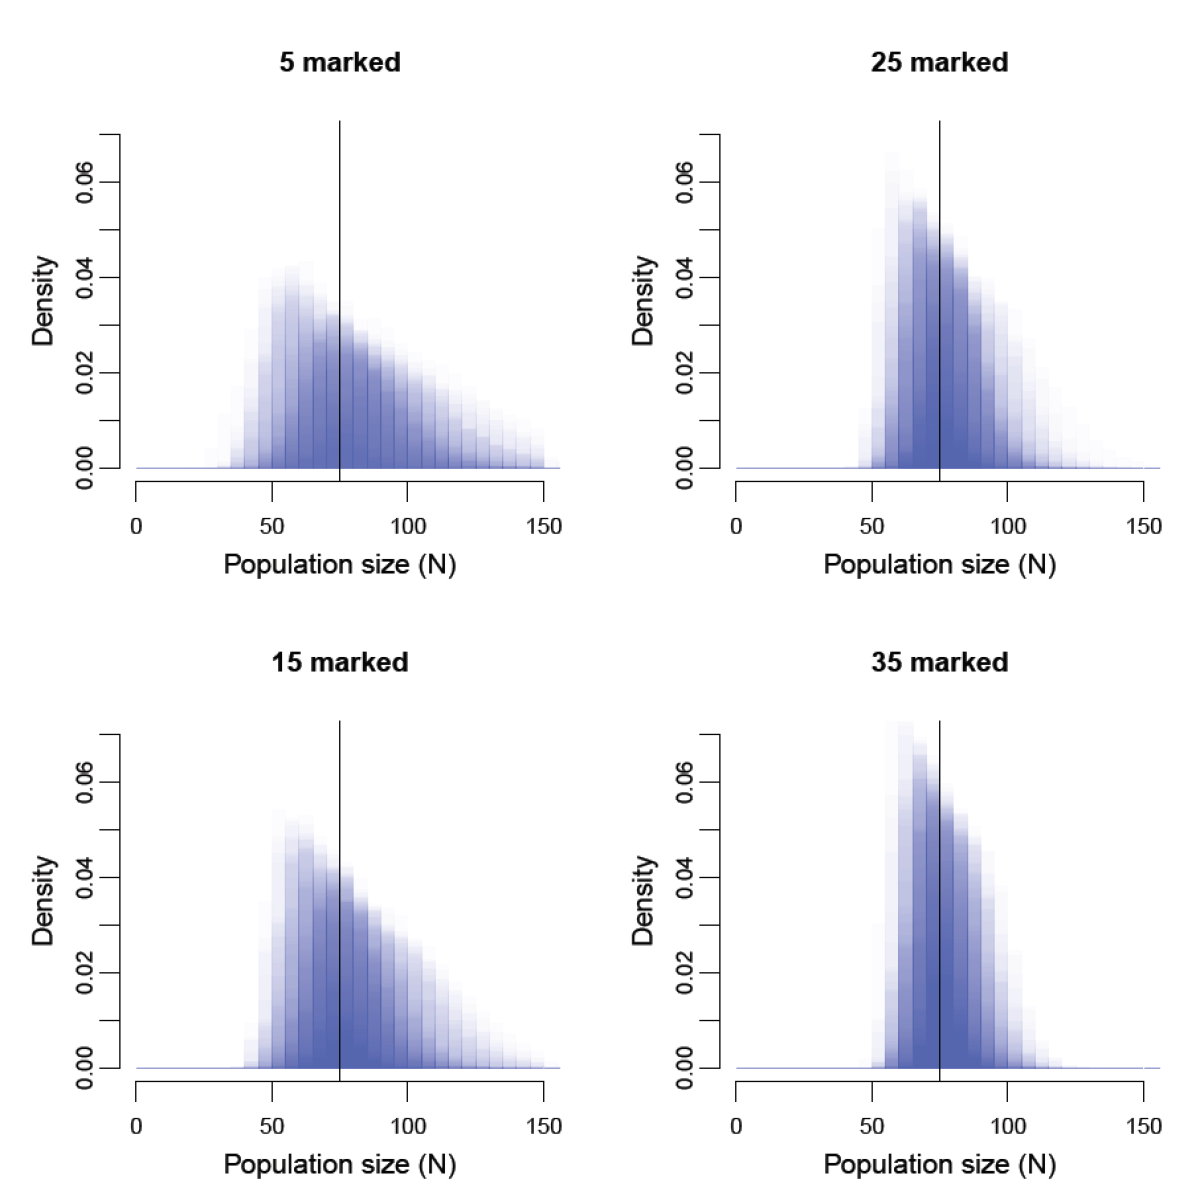
\includegraphics[width=4in,height=4in]{Ch15/figs/Nposts2.png}
  \caption{Overlaid posterior distributions of $N$ from 100 simulations
    for four levels of marked individuals.}
  \label{partialID.fig.nposts}
\end{figure}

Without any marked individuals in the population, the posterior distribution of $N$ turned out to be highly skewed, but its mode was still an approximately unbiased point estimator of $N$. As anticipated, posterior precision increased substantially with the proportion of marked individuals (Tab. \ref{partialID.tab.sim} and Fig. \ref{partialID.fig.nposts}). The posterior mode was approximately unbiased as a point estimator, and the relative root-mean squared error decreased from 0.246 when no individuals were marked to 0.085 when 35 individuals were marked (Tab. \ref{partialID.tab.sim}). Coverage was nominal for all values of $m$ and posterior skew greatly diminished with increasing $m$(Tab. \ref{partialID.tab.sim}).


\begin{table}[ht]
\centering
\caption{Posterior mean, mode, and associated relative RMSE for simulations in
  which $m$ of $N$=75 individuals were marked. One hundred simulations of each case were conducted. }
\begin{tabular}{llrrrrr}
     \hline
     &	Parameter    &	Mean   &	rRMSE  & Mode   & rRMSE &	BCI    \\
     \hline
 m=0 &	$N$          &	85.866 &    0.259 & 77.720 &    0.242 & 0.950  \\
     &	$\lambda_0$  &	0.506  &	0.180 &	0.488  &	0.182 &	0.960  \\
     &	$\sigma$     &	0.495  &	0.115 &	0.486  &	0.113 &	0.960  \\
     \hline
 m=5 &	$N$          &	80.898 &    0.184 & 76.360 &    0.182 & 0.970  \\
     &	$\lambda_0$  &	0.510  &    0.178 & 0.494  &    0.180 & 0.950  \\
     &	$\sigma$     &	0.496  &    0.089 & 0.488  &    0.086 & 0.970  \\
     \hline
 m=15&	$N$          &	79.028 &    0.148 & 76.250 &    0.147 & 0.950  \\
     &	$\lambda_0$  &	0.508  &    0.163 & 0.494  &    0.164 & 0.950  \\
     &	$\sigma$     &	0.496  &    0.073 & 0.492  &    0.071 & 0.970  \\
     \hline
 m=25&	$N$          &	77.765 &    0.114 & 75.810 &    0.113 & 0.950  \\
     &	$\lambda_0$  &	0.511  &    0.153 & 0.498  &    0.157 & 0.950  \\
     &	$\sigma$     &	0.496  &    0.067 & 0.493  &    0.065 & 0.940  \\
     \hline
 m=35&	$N$          &	76.446 &    0.085 & 74.900 &    0.085 & 1.000  \\
     &	$\lambda_0$  &	0.513  &    0.142 & 0.501  &    0.144 & 0.950  \\
     &	$\sigma$     &	0.497  &    0.056 & 0.493  &    0.057 & 0.940  \\
 \hline
\end{tabular}
\label{partialID.tab.sim}
\end{table}

As we saw in the previous chapter, the spatial correlation in unmarked counts can be sufficient to obtain estimates of movement and detection parameters. However, only marked and thus identifiable individuals provide us with direct information about these parameters and may well dominate estimates. 
To single out the contribution of marked and unmarked individuals to parameter estimates, we re-ran the same simulations but let $\sigma$ and $\lambda_0$ be updated based solely on the data of marked individuals. Results are summarized in Tab. \ref{partialID.tab.sim2}.
We see that if we update $\lambda_0$ and $\sigma$ based on marked individuals only, estimates of these parameters are more biased and less precise. For estimates of $N$, especially for $m$= 5 and $m$ = 15, we observe a stronger positive bias, lower accuracy and considerably lower BCI coverage as compared to when both marked and unmarked individuals contribute to parameter estimates (Tab. \ref{partialID.tab.sim2}). Thus, unmarked individuals do actually contribute noticeably to estimating model parameters. 

\begin{table}[ht]
\centering
\caption{Posterior mean, mode, and associated relative RMSE for simulations in
  which $m$ of $N$=75 individuals were marked and unmarked individuals 
  did not contribute to estimating $\lambda_0$ and $\sigma$. 
  One hundred simulations of each case were conducted. }
\begin{tabular}{llrrrrr}
\hline
     &	Parameter    &	Mean   &	RMSE  &	Mode   &	RMSE &	BCI    \\
     \hline
 m=5 &	$N$          &	88.621 &	0.369 &	83.139 &	0.421 &	0.810  \\
     &	$\lambda_0$  &	1.255  &	1.247 &	0.606  &	1.148 &	0.950  \\
     &	$\sigma$     &	0.472  &	0.252 &	0.426  &	0.333 &	0.910  \\
     \hline
 m=15&	$N$          &	81.031 &	0.192 &	78.361 &	0.175 &	0.820  \\
     &	$\lambda_0$  &	0.535  &	0.281 &	0.476  &	0.284 &	0.970  \\
     &	$\sigma$     &	0.503  &	0.109 &	0.490  &	0.107 &	0.940  \\
     \hline
 m=25&	$N$          &	78.206 &	0.129 &	76.594 &	0.123 &	0.920  \\
     &	$\lambda_0$  &	0.531  &	0.204 &	0.496  &	0.202 &	0.960  \\
     &	$\sigma$     &	0.497  &	0.081 &	0.489  &	0.084 &	0.950  \\
     \hline
 m=35&	$N$          &	76.833 &	0.099 &	75.422 &	0.096 &	0.940  \\
     &	$\lambda_0$  &	0.528  &	0.192 &	0.505  &	0.186 &	0.940  \\
     &	$\sigma$     &	0.499  &	0.069 &	0.493  &	0.070 &	0.960  \\
 \hline
\end{tabular}
\label{partialID.tab.sim2}
\end{table}


\section{Incorporating telemetry data}
\label{partialID.sec.telemetry}
As we expected, parameter estimates of spatial mark-resight models get better the more marked individuals we have in our study population. While this is great advice in theory, it may not be very helpful in practice, especially when dealing with animals that are hard or somewhat dangerous to capture, such as large carnivores. Oftentimes, studies involving the physical capture of such animals will employ telemetry tags in order to learn about the study species' spatial ecology and behavior. In the context of spatial mark-resight models, the actual locational data collected by telemetry tags can provide detailed information on individual location and movement, and being able to incorporate this information directly into the SMR model should improve estimates of these parameters, especially when resighting information is sparse.

So how could we combine resighting data and telemetry data in a unified mark-resight model? Recall that the basic SCR model underlying all the SMR models we discuss here uses a half-normal detection function.
By using this function, we can relate the parameters $\sigma$ and ${\bf s}_{i}$ directly to those from a bivariate normal model of space usage, with mean = ${\bf s}_{i}$, and variance-covariance matrix $\Sigma$, where the variance in both dimensions is $\sigma^2$ and the covariance is 0. Ordinarily, these parameters are estimated directly from the spatial distribution of individual recaptures/resightings. Telemetry data, however, provide more detailed information on individual location and movement, since the resolution and extent of the data are not limited by the trapping grid and potentially more locations can be accumulated through telemetry than resighting (depending on the monitoring frequency and resighting rates of individuals).  

By assuming that the $R$ locations of individual $i$, ${\bf l}_{i}$ (consisting of a pair of x and y coordinates, $l_{ix}$ and $l_{iy}$), are a bivariate normal random variable:
\[
{\bf l}_i\sim {\mbox Normal}_2 ({\bf s}_i,\Sigma)
\]
we can estimate $\sigma$ as well as ${\bf s}_{i}$ for the collared individuals directly from telemetry locations, using their full conditional distributions:
\[
[\sigma|{\bf l},{\bf s}] \propto \left\{\prod_{i=1}^m \prod_{r=1}^R \frac{1}{2 \pi \sigma^2} {\exp}\left(-1/2 \left[ \frac {(l_{irx}-s_{ix})^2} {\sigma^2} + \frac{(l_{iry}-s_{iy})^2}{\sigma^2} \right]\right)\right\}*[\sigma] 
\] 
and
\[
[{\bf s}_i|{\bf l},\sigma] \propto \left\{\prod_{r=1}^R \frac{1}{2 \pi \sigma^2} {\exp}\left(-1/2 \left[ \frac {(l_{irx}-s_{ix})^2} {\sigma^2} + \frac{(l_{iry}-s_{iy})^2}{\sigma^2} \right]\right)\right\}*[{\bf s}_{i}] 
\]

Under the standard mark-resight assumption that marked individuals are a representative sample of the population, the estimate of $\sigma$ can be applied for the entire population. For the unmarked individuals ${\bf s}_{i}$ are estimated as described before conditional on their latent encounter histories. 

{\bf R} makes it easy to implement the update of $\sigma$ and ${\bf s}_i$ based on telemetry data and the above described full conditionals within our existing MCMC algorithm. We replace the current updating step for $\sigma$ with: 
{\small
\begin{verbatim}
#ntot = number of telemetry-tagged individuals
#locs = list of length ntot; each element is a matrix 
#with telemetry locations
#telID = vector with identifier for telemetry-tagged
#individuals

sigma.cand <- rnorm(1, sigma, delta[1])
if (sigma.cand > 0) {

llsig<-llsig.cand<-rep(NA, ntot) 

for (x in 1:ntot) {
lls[x]<-sum(dmvnorm(x=locs[[x]],mean=c(S[telID[x],1],S[telID[x],2]), 
			sigma=cbind(c(sigma^2,0), c(0,sigma^2)), log=T))   
lls.cand[x]<-sum(dmvnorm(x=locs[[x]],mean=c(S[telID[x],1],S[telID[x],2]), 
	sigma=cbind(c(sigma.cand^2,0), c(0,sigma.cand^2)), log=T))   
	}
   if(runif(1) < exp( sum(lls.cand)  - sum(lls) ) ){
    sigma<-sigma.cand
    lam <- lam0*exp(-(D*D)/(2*sigma.cand*sigma.cand))
					}
			}
\end{verbatim} 
}
For the ${\bf s}_i$ we use an analogous updater for the telemetry-tagged individuals and the regular updater for individuals without associated telemetry location information. A full example can be found in the {\bf R} package {\tt scrbook}, by calling {\tt scrPID.tel}. Note that not all marked individuals need to be telemetry-tagged, but telemetry data used on the model should correspond to the period over which resighting surveys were conducted (as we discussed in Chapt. \ref{chapt.scr0}, both the ${\bf s}_i$ and $\sigma$ should only be interpreted against the specific sampling period). Further, this approach of incorporating telemetry data into a spatial mark-resight model can easily be extended to update $\sigma$ and ${\bf s}$ conditional on both resighting and telemetry data and applies equally to regular SCR models where all individuals are identifiable. 

{\flushleft \bf Example: Raccoons on the Outer Banks of North Carolina }
 
\citet{sollmann_etal:inprepecology} applied a spatial mark-resigh model with telemetry data to a camera-trap and radio-telemetry data set from the raccoon population on South Core Banks, a barrier island within Cape Lookout National Seashore, North Carolina. Between May and September 2007, 131 raccoons were marked with dog collars and large individually numbered cattle tags; 44 of these tagged individuals were equipped with radio collars. Collared individuals were located using a VHF receiver and antenna, and their locations were estimated approximately weekly. Twenty camera traps  were set up along the length of South Core Banks and camera trapping data collected between October 1 2007 to January 22 2008 constituted the resighting data in this analysis. During this period 104 marked individuals, 38 radio-collared, were alive and available for resighting with camera traps. 

\begin{figure}[ht]
  \centering
  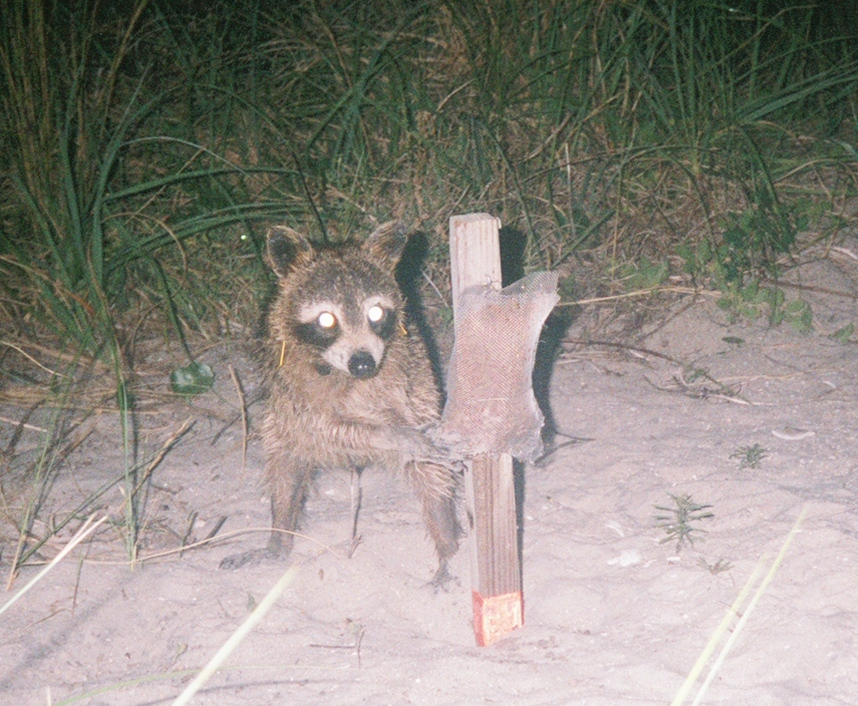
\includegraphics[width=4in]{Ch15/figs/Raccoon_pic.png}
  \caption{Camera trap picture of a raccoon marked with a cattle tag that cannot be read to determine individual identity. Taken on South Core Banks, North Carolina.
({\it Photo credit: Arielle Parsons})}
  \label{partialID.fig.raccoon}
\end{figure}

The state-space ${\cal S}$ was defined as the entire area of South Core Banks island. A change in the number of photocaptures over the course of the study suggested a variation of detection rate with time. Since date recording in cameras malfunctioned, photographic records could only be assigned to the time interval between subsequent trap checks, and these intervals between checks are referred to as sampling occasions. These occasions ranged from 2 to 43 days; $\lambda_0$ was standardized to 7-day intervals and allowed to change with sampling occasion. Since not all pictures of marked raccoons could be identified to the individual level, the authors applied the correction factor $c$ as described in sec. \ref{partialID.sec.IDrate}, estimated separately for each occasion. 

Camera-traps recorded 117 pictures of unmarked raccoons, 33 pictures of 18 marked and identifiable raccoons, and 49 records of marked but not individually identifiable individuals (Fig. \ref{partialID.fig.raccoon}). An average of 16.32 telemetry locations (SD 4.91) were collected for each of the 38 collared individuals. Raccoon abundance on the island was estimated at 186.712 (SE 14.810) individuals, which translated to a density of 8.291 (SE 0.658) individuals per $km^2$. Parameter estimates are listed in Tab. \ref{partialID.tab.raccoons}. 

\begin{table}%[hb]
\centering
\caption{Summary statistics of parameter estimates from spatial mark-resigh model for raccoon camera trapping and telemetry data. Baseline trap encounter rate $\lambda_0$ was standardized to 7-day intervals; $\lambda_0$ and the probability of identifying a picture of a marked individual, $c$, were allowed to vary among the 6 sampling occasions (t); $\sigma$ is estimated from telemetry data of 38 radio-collared individuals.}
\begin{tabular}{lrrrrr}
\hline
   &	Mean (SE) &	2.5\% &	50\%	& 97.5\% \\
 \hline
$\sigma$	& 0.491 (0.010)	& 0.472	& 0.491	& 0.512 \\
$\lambda_0$ (t=1)	& 0.237 (0.045) & 0.158 & 0.234 & 0.335 \\
$\lambda_0$ (t=2)	& 0.397 (0.081)	& 0.257	& 0.391	& 0.573 \\
$\lambda_0$ (t=3)	& 0.108 (0.028) & 0.061 & 0.105	& 0.170 \\
$\lambda_0$ (t=4)	& 0.296 (0.073)	& 0.174	& 0.289	& 0.459 \\
$\lambda_0$ (t=5)	& 0.032 (0.011)	& 0.015	& 0.030	& 0.056 \\
$\lambda_0$ (t=6)	& 0.031 (0.009)	& 0.016	& 0.030	& 0.052 \\
$c$ (t=1)	& 0.545 (0.085)	& 0.377	& 0.546	& 0.709 \\
$c$ (t=2)	& 0.389 (0.112)	& 0.184	& 0.385	& 0.616 \\
$c$ (t=3)	& 0.294 (0.107) & 0.110	& 0.286	& 0.523 \\
$c$ (t=4)	& 0.375 (0.162)	& 0.099	& 0.364	& 0.710 \\
$c$ (t=5)	& 0.375 (0.161)	& 0.099	& 0.364	& 0.709 \\
$c$ (t=6)	& 0.300 (0.138)	& 0.075	& 0.287	& 0.600 \\
$N$	& 186.712 (14.810) & 162 & 185	& 220 \\
$D$	& 8.291 (0.658)	& 7.194	& 8.215	& 9.769 \\
 \hline
\end{tabular}
\label{partialID.tab.raccoons}
\end{table}

In this study, although a large number of raccoons were tagged, photographic data of these tagged individuals were surprisingly sparse. Analysis of the photographic data set without the telemetry data did not render usable estimates as parallel Markov chains did not converge. One reason for the relatively sparse data was the camera trap study design: traps were spaced on average 1.77 km apart, which is about 3.5 times $\sigma$. Consequently, very few individual raccoons were photographed at more than one trap. Under these circumstances, the telemetry data provide the necessary spatial information to estimate $\sigma$ and the activity centers of individual animals and thus make other model parameter estimable. Similarly, in a camera-trapping study on Florida panthers (\emph{Puma concolor coryi}), \citet{sollmann_etal:inprepjapplecol}, including telemetry data from the 3 individuals that were collared and known to use the study area resulted in density estimates with considerably higher precision as compared to preliminary estimates \emph{without} telemetry location data, reducing the width of the 95 \% BCI by about 60 \%. Such improvements in precision of estimates is especially important when we are interested in changes in the population over time. 


\section{Summary and Outlook}
In this chapter we combined SCR models and the spatial model for unmarked populations to derive a spatial mark-resight model, which accomodates that part of the population is individually identifiable, usually through artificial tags. The basic model with known number of marked individuals and 100 \% individual identification of marked is easily modified for situations where the number of marked individuals is unknown, or where marked animals can sometimes not be identified to individual level. As expected, having marked individuals in the study population improved accuracy and precision of parameter estimates when compared to fully unmarked populations, but we also saw that the spatial counts of unmarked individuals still contribute information to parameter estimates. Finally, we present an approach of how to incorporate telemetry location data into the spatial mark-resight model to inform estimates of $\sigma$ and activity centers. Especially for difficult-to-study, cryptic species where often only a small sample of the population can be tagged this enables researchers to make optimal use of all existing data and obtain robust density estimates without the need for additional invasive methods. Just as SCR, the spatial mark-resight model framework is flexible to account for a variety of factors that may influence individual movement and detection, as well as survey-related parameters, and we saw one example for the Canada geese, where $\sigma$ was sex-sepcific.
 
Spatial mark-resight models are a fairly new development and much remains to be explored. We mentioned the assignment of marked but unidentified records to actual marked individuals based on their spatial location, which provides some (though imperfect) information of their identity (sec. \ref{partialID.sec.IDrate}). Similarly, records where the marked status cannot be determined could potentially be included in the model as some form of overall correction factor on detection. GPS telemetry devices and their ability to collect location data with much higher frequency offer the opportunity to assign records of collared animals to individuals based on how close to a given camera the collared individuals were, both in space and time. In this scenario, individual identity itself could be expressed probabilistically, leading to an SMR model accouting for potential misidentification. All these possible extensions can tailor SMR models to specific survey techniques. As such, the approach is applicable to a wide range of population estimation problems when dealing with animals that cannot be identified based on natural marks. 








 